\subsection{Geographic Engine}\label{comp:geographicEngine}
The Geographic Engine is responsible for calculating the approximative waiting time for a passenger, and for computing the corresponding zone of a location. Internally it is composed of the following components each with a precise job:
\begin{itemize}
	\item \textit{WaitingTimeCalculator}: when it receives a call, it forwards the source and the destination to a Google Maps Web Service which computes the approximative traveling time.
	\item \textit{ZoneCalculator}: it is responsible for storing the geographic definition of the zones and compute if a location is valid, and if it is in which zone is located. To do that it needs the Google Maps Web Service for the activity geocoding, which means to get geographic coordinates from an address.
\end{itemize}
\begin{figure}[H]
	\centering
	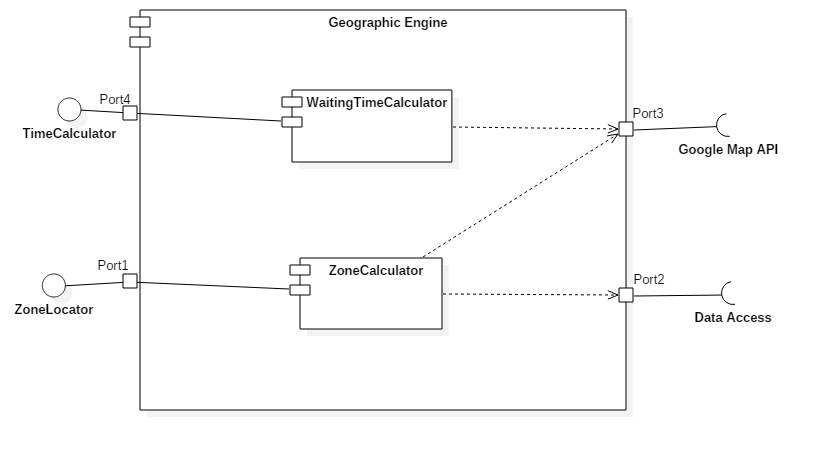
\includegraphics[scale=0.5]{../"Analysis Documents"/components/geographicEngine}
	\label{fig:geographicengine}
	\caption{Geographic Engine internal structure}
\end{figure}
\subsubsection{Provided interfaces}
\begin{table}[H]
	\begin{longtable}{| p{0.3\textwidth} | p{0.3\textwidth} | p{0.4\textwidth} |}
		\hline
		\textbf{Provided Interface} & \textbf{Dedicated user} & \textbf{Description} \\ \hline
		TimeCalculator & Ride Manager component & Given a source location and a destination, it calculates an approximative waiting time \\ \hline
		ZoneLocator & Taxi Manager, Queue Manager and Ride Manager components & It calculates the corresponding zone of a given location if it is valid (being valid means to be inside the city) \\ \hline
	\end{longtable}
	\caption{Geographic Engine: provided interfaces}
	\label{tab:geographicengine:providedInterfaces}
\end{table}
\subsubsection{Required interfaces}
\begin{table}[H]
	\begin{longtable}{| l | p{.80\textwidth} |}
		\hline
		\textbf{Required Interface} & \textbf{Description and usage} \\ \hline
		Google Maps API & Used for the activity of geocoding and for calculating the approximative travel time \\ \hline
		DataAccess & Retrieve the information about taxi zones \\ \hline
	\end{longtable}
	\caption{Geographic Engine: required interfaces}
	\label{tab:geographicengine:requiredInterfaces}
\end{table}
